\chapter{Waving Grass}

% GPU gems 1 chapter 7

A completely static terrain would appear quite lifeless. Some foliage
gently swaying in the wind would make the landscape seem more idyllic
and therefore we chose to add waving grass straws. Some considered
rendering techniques for grass were:

\begin{itemize}
\item Rendering grass straw textures on quads. This allows us to
  render several grass straws while only having to process 4
  vertices. Letting it wave in the wind is also easy as that only
  means moving the 2 top vertices. A problem however is that the
  illusion breaks down when viewed from above or on steep cliffs.
\item Modeling each grass straw. This technique allows for very
  flexible grass with correct lighting. It is however very expensive
  to process all the vertices, so it is ususally used in conjunction
  with the above method for far away grass.
\item Rendering a volume texture containing the grass straws.
\end{itemize}

We opted for grass drawn onto quads, since it is easy to draw a quad
in the scene and grass textures are easy to come by. However the
entire landscape can not simply be covered with millions of quads, as
that would be extremely expensive to render, so there are some design
decisions to be made. Another problem with this technique is that part
of the grass texture is transparent, and transparency is not easy to
render in the OpenGL 2.1 pipeline. A solution would be \emph{depth
  peeling} or \emph{z-sorting} the straws, but for our purpose we
propose a much simpler method in the
\hyperref[sec:transparency]{Handling Transparency subsection}.

The basis of the grass implementation is
\citebook{chapter~7}{983868}. Here they propose to draw the quads in
star patterned grass objects, to achieve a grass effect independent of
the cameras line of sight. Our implementation does the same, but
allows the user to specify how many quads should be used pr. star
object. Setting this to 1 effectively disables the star pattern and
simply renders random quads of grass straws instead.

\section{Placing the grass}

As stated earlier we cannot simply draw the grass everywhere without
incurring a huge performance penalty, so instead we focus on drawing
the grass around the camera. We choose to draw it in a square around
the camera, but other shapes should be possible.

% explain algorithm

On \reffig{fig:grassTranslation} the basics of the algorithm can be
seen. We need to translate the grass bounding box centered around
origo to the camera's position. We can not simply use the vector from
origo to the camera, since that would make the grass straws float
along with the camera. Instead we need the global position of the
quads to be moved up to the camera with a step size equal to the
length of the bounding box' side. From the camera this would create
the effect that quads exiting the camera bounding box on one side
would reappear on the other side. In practice this isn't visible from
the camera and the illusion of individuel grass straws is
preserved. The following equation expresses the this desire.

\begin{displaymath}
    -halfSize \le position + size * n - eye \le halfSize, n \in N \\
\end{displaymath}

Focussing on the left hand side of the equation and remembering that
$n$ should be an integer, $n$ can be calculated as

\begin{displaymath}
  \begin{array}{l}
    -halfSize \le position + size * n - eye \\
    \Updownarrow \\
    (eye - halfSize - position) / size \le n \\
    \Updownarrow \\
    n = \lceil (eye - halfSize - position) / size \rceil \\
    \Updownarrow \\
    n = \lceil (eye - position) / size - 0.5 \rceil \\
  \end{array}
\end{displaymath}

Now the new position of the grass straw is simply calculated by 

\begin{displaymath}
  newPos = position + size * n
\end{displaymath}

An added benefit to this approch is that even though the grass is
dynamically placed, it is deterministic and is always placed the
same. This means that if a user is exploring the terrain and returns
to a previously visited area, the grass will be placed the same way.

% And placing it in front of the camera

The grass objects have now succesfully been placed inside the bounding
box around the camera, as can be seen on
\reffig{fig:grassTranslation}. However most of the straws still are
not inside the frustum. A small trick can be applied to move more of
the grass up in front of the camera. Instead of placing the grass
around the camera, it can be placed at a position in front of it,
relative to the cameras current direction. Since at least half the
grass bounding box will be behind the camera, we choose to move the
bounding box by the $halfSize$ multiplied by the normalized camera
direction. This places the center of the grass in front of the camera,
but the border will always be behind the camera. The result is many
more grass straws on the screen at the same vertex processing cost.

\begin{figure}
  \centering
  \begin{tikzpicture}[y=0.5cm, x=.5cm,font=\sffamily]
    \draw (0,0) -- coordinate (x axis mid) (10,0);
    \draw (0,0) -- coordinate (y axis mid) (0,5);

    \draw (-2,-2) -- coordinate (x axis mid) (-2,2);
    \draw (2,-2) -- coordinate (x axis mid) (2,2);
    \draw (2,2) -- coordinate (x axis mid) (-2,2);
    \draw (2,-2) -- coordinate (x axis mid) (-2,-2);

    \draw (3,0) -- coordinate (x axis mid) (3,4);
    \draw (7,0) -- coordinate (x axis mid) (7,4);
    \draw (7,4) -- coordinate (x axis mid) (3,4);
    \draw (7,0) -- coordinate (x axis mid) (3,0);

    \draw (-1.5,2.2) -- coordinate (x axis mid) (2.5,3.8);
    \draw (2,3.8) -- coordinate (x axis mid) (2.5,3.8);
    \draw (2.15,3.5) -- coordinate (x axis mid) (2.5,3.8);
    
    \draw (2.5,-1.8) -- coordinate (x axis mid) (6.5,-0.2);
    \draw (6,-0.2) -- coordinate (x axis mid) (6.5,-0.2);
    \draw (6.15,-0.5) -- coordinate (x axis mid) (6.5,-0.2);

  \end{tikzpicture}
  \caption{The translation of the grass bounding box from origo out to the camera.}
  \label{fig:grassTranslation}
\end{figure}


% creation and one draw call

Since grass placed anywhere will now be translated to the camera, we
can create it anywhere we like. More importantly all the quads of
grass straws can now be drawn with one single draw call, and the
vertex shader will translate it to the camera. This removes a major
overhead we would have had if all quads were drawn individually. \\

% Placing it on the heightmap and normal lookup

Next we must translate the grass objects along the y-axis to place
them on the terrain, instead of below or above. Since we're
continuesly translating the grass quads, we won't know their correct
height at creation time and must therefore look it up in the vertex
shader. From grass' xz-position a texture coordinate can be calculated
and used to lookup into the heightmap texture, where we can find the
correct height for the grass. To ensure that the terrain and grass are
equally lit, we use the same procedure to lookup into the heightmaps
normalmap.

% not on sand or snow.

The last part of the grass placement is to keep it off the sand, snow
and steep cliffs. To this end we pass along the center of the grass
straw to the vertex shader. The center is then subjected to the same
translations as the vertex position. Wether or not the grass straws
should be visible can then be estimated from the height of the
center. If the center is too low the grass is on sand and should not
be visible, likewise if the center is too high it is on snow. A
similar scheme is used for deciding if the grass is placed on cliff,
where the angle of the normal compared to the upvector is the deciding
factor.

The reason for using the center of the grass objects is that while one
side of the quad may be placed perfectly legal, the other side could
be placed on sand or snow. In order to collapse the grass objects we
needed a constant variable across the objects and that is the center.


\section{Waving in the wind}

Our animation algorithm is the same as the one proposed in
\citebook{section~7.4.4}{983868}, where the grass objects center is
used to create \emph{local chaos}. This means that textures are
minimally distorted, since the vertices always have the same distance
to their neighbours, and the local chaos creates a more natural wave
effect. Of the two cons to the approach desribed in
\citebook{section~7.4.4}{983868}, only one of them applies to our
implementation. The first con, which is that extra uniform data is
required to hold the center of the grass object, does not apply in
this case, since the center was needed anyway. The second con does
apply to our shader, namely that the complexity of the animation
algorithm is limited in order to minimize the cost of the shader. The
wave therefore is just a simple cosine function applied to the two top
vertices, distinguished by their texture coordinate.


\section{Handling Transparency}\label{sec:transparency}

% Discarding seethrough texture (how to avoid z sorting and rendering
% everything with one draw call)

With the grass placed on the terrain, texture transparency needs to be
handled. Our grass straw texture can be seen in
\reffig{fig:grassStraws}. Since all grass objects are drawn with one
draw call, z-sorting every frame is not an option. Instead the
transparency issue is completely ignored, by only rendering completely
opaque fragments or discarding transparent fragments. This is done in
the fragment shader, where colors with alpha values below a certain
value are simply discarded. The reason for not just discarding
everything with alpha values stictly below one is that mipmapping has
to be taken into account. If two opague and two transparent pixels are
combined in a lower mipmap layer, this would yield an alpha of 0.5,
but the fragment should perhaps still be rendered. In practice we
found that discarding alphas below 0.6 works well with our grass straw
texture.

\begin{figure}
  \centering
  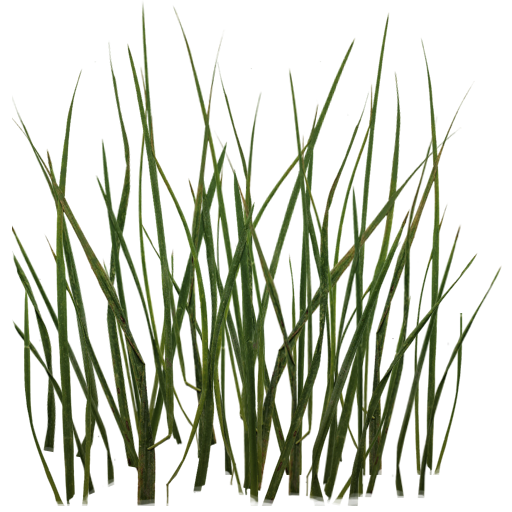
\includegraphics[width=5cm]{grassStraw}
  \caption{The grass straws.}
  \label{fig:grassStraws}
\end{figure}

% Simple diffuse lighting, no specular.

%%% Local Variables:
%%% mode: latex
%%% TeX-master: t
%%% TeX-PDF-mode: t
%%% End:
